\chapter{Design}

\begin{longtabu} to \linewidth{@{}l l l X[j]@{}}
    Version &    Dato &    Ansvarlig &    Beskrivelse\\[-1ex]
    \midrule
    
\label{version_Systemark}
\end{longtabu}

\section{Indledning}

  
\section{Hardware arkitektur}
I følgende afsnit beskrives hvordan blodtryksmåler systemet og nogle af dets delkomponenter er opbygget.
\\
\begin{figure}[H]
	\centering
	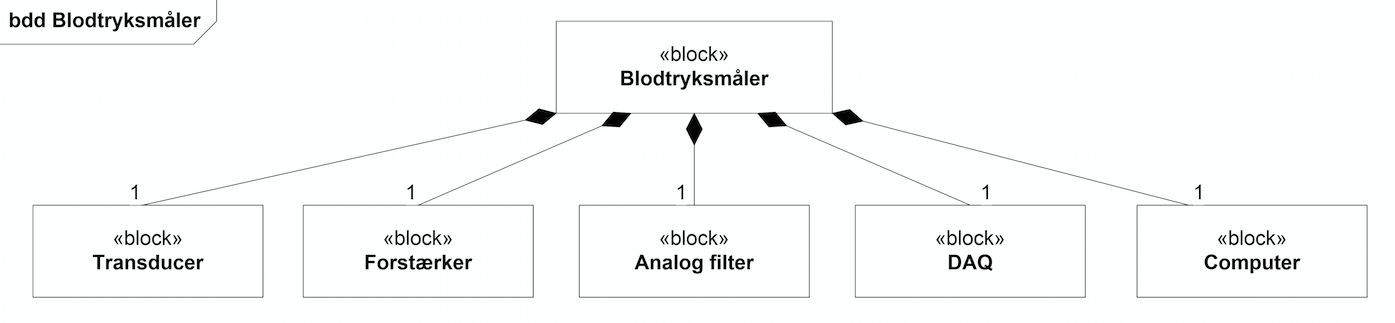
\includegraphics[width=1\textwidth]{Figurer/BDD}
	\caption{Blokdiagram for blodtryksmåler systemet.}\label{labelpic}
\end{figure}

Ud af blokdiagrammet kan man se at blodtryksmåler systemet består af en transducer, en forstærker, et analogt filter, en DAQ og en computer.\\
\begin{figure}[H]
	\centering
	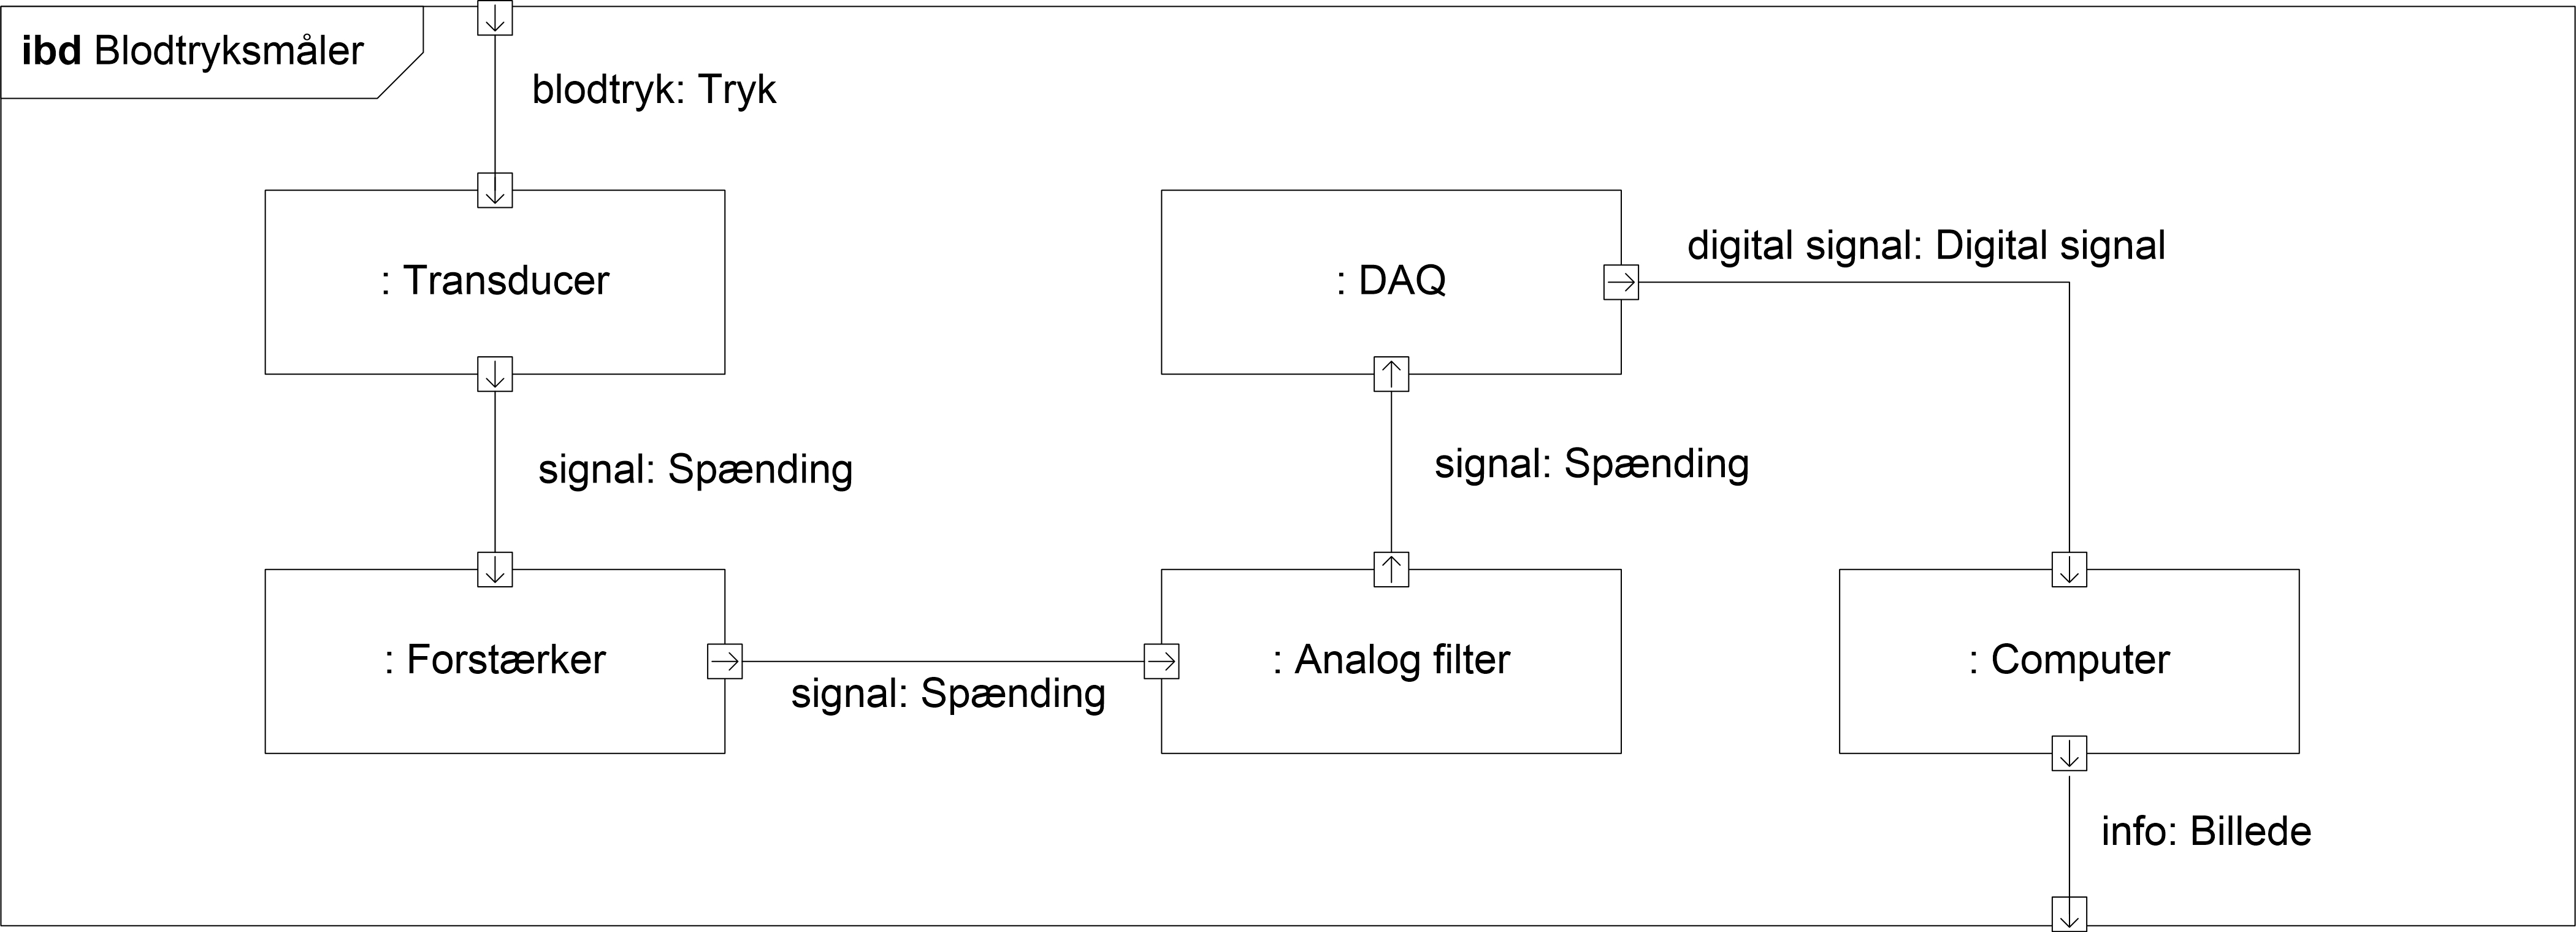
\includegraphics[width=1\textwidth]{Figurer/IBD}
	\caption{Internt blok diagram for blodtryksmåler systemet.}\label{labelpic}
\end{figure}

Ud af det interne blok diagram kan ses det at blodtrykket i form af det målte tryk kommer ind i transduceren. Transduceren som omformer det målte tryk til et spændingssignal, sender signalet vidre til forstærkeren. Fra forstærkeren sendes signalet over i det analoge filter og derfra ind i DAQ'en. Endeligt sendes det digitale signal fra DAQ'en over i en computer, der fortolker signalet som et billede, der vises til omverdenen.

\subsection{Design af forstærker}
Forstærkeren er designet med tanke på, at det er meget små spændinger der arbejdes med. Grundet dette, er en almindelig operationsforstærker fravalgt, da dens reelle indgangsimpedans er for lille. En Instrumentationsforstærkers indgangsimpedans i den virkelige verden, er højere, og den kan dermed opfange meget små signaler så som blodtryk.\\
Vejleder rådede herefter til at projektgruppen brugte instrumentationsforstærkeren INA114. Forstærkerens design kan ses på figur X.\\ 
\begin{figure}[H]
	\centering
	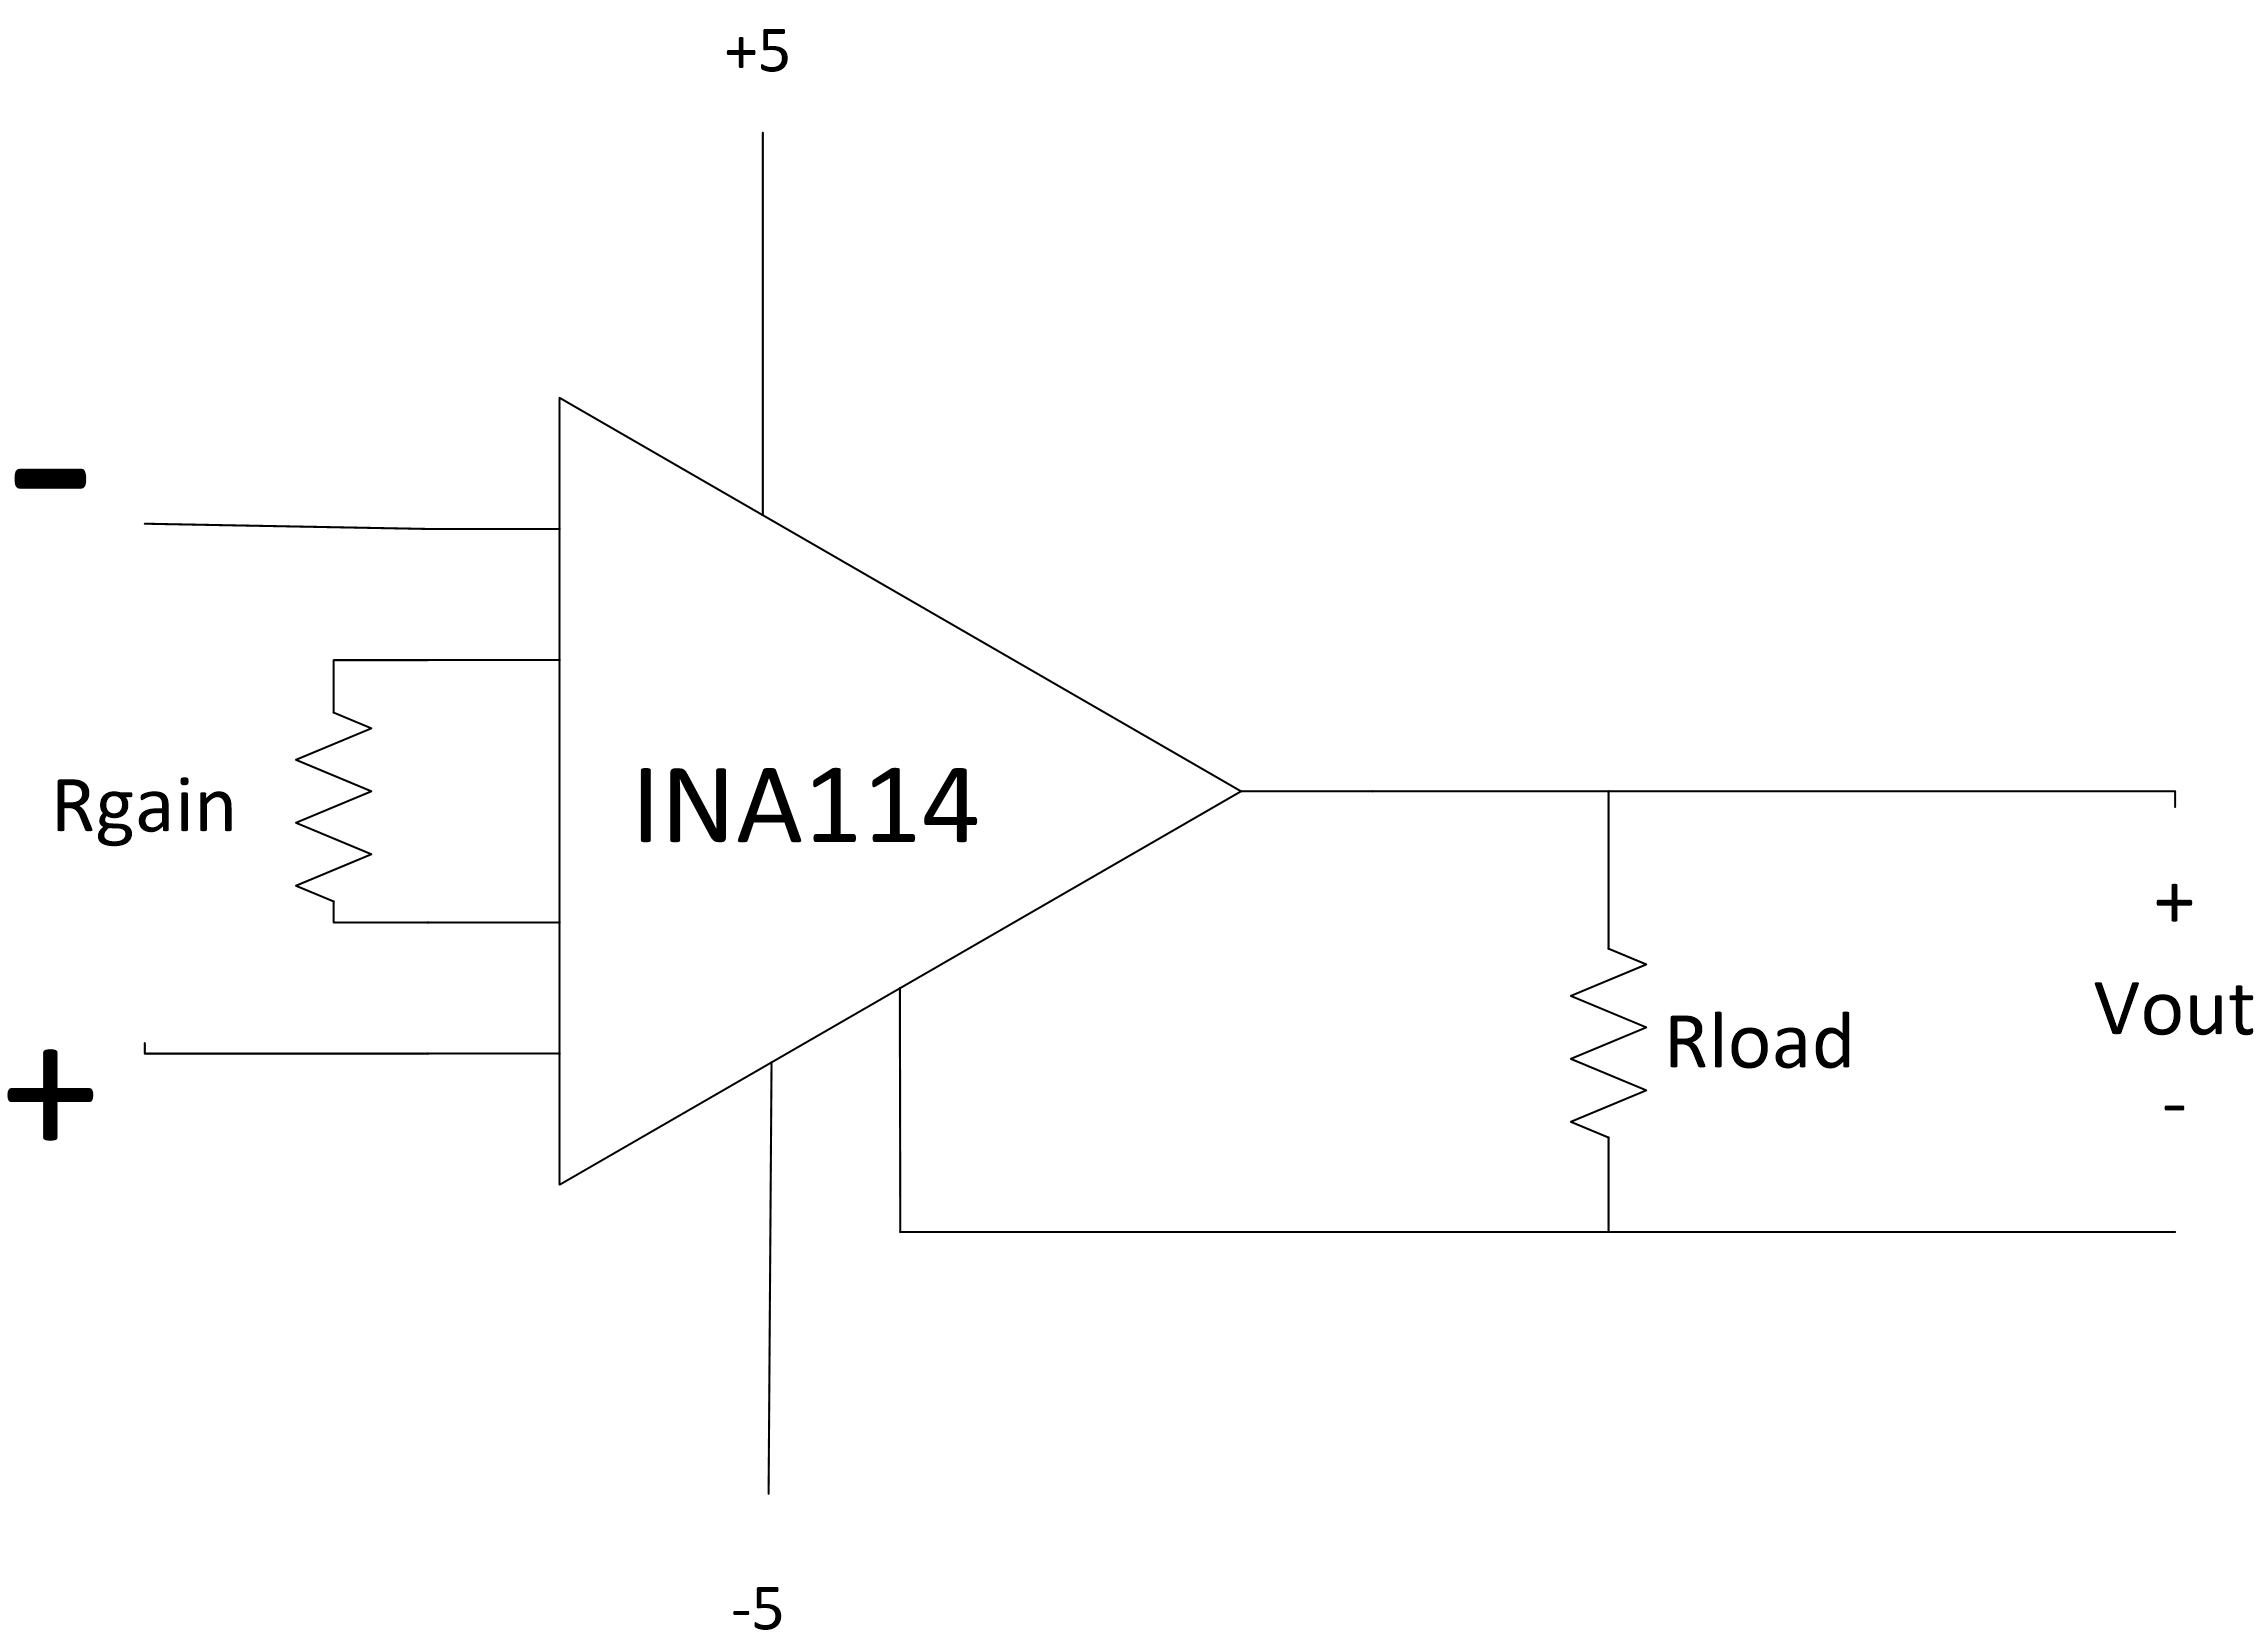
\includegraphics[width=1\textwidth]{Figurer/Forstaerker}
	\caption{Der overordnede design af forstærkeren.}\label{labelpic}
\end{figure}
*Rgain* er modstanden, som bestemmer, hvor meget forstærkning, instrumentationsforstærkeren skal give og *Rload* er den belastning, der kommer efter kredsløbet. I dette tilfælde, er det, det analoge filter. For at finde *Rgain’s* størrelse, kræver det, at der vides, hvor meget forstærkning der er brug for. Dette findes, ved at bestemme den maksimale spænding, som transduceren kan give, i en blodtrykssituation. Dette regnestykke kan ses realiseret i ligning x.\\
\begin{figure}[H]
	\centering
	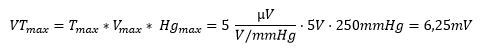
\includegraphics[width=1\textwidth]{Figurer/LigningSara}
\end{figure}

Spændingen ønskes at skaleres op til DAQ’ens dynamikområde, som ligger omkring de 5V. Forstærkningsfaktoren udregnes ved simpel brøkregning. \\

\begin{figure}[H]
	\centering
	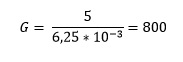
\includegraphics[width=1\textwidth]{Figurer/ligningtilgain}
\end{figure}

INA114’s datasheet giver en ligning for udregning af forstærkning. Da forstærkningen er kendt, omskrives denne ligning, så modstanden *Rgain’s* værdi i stedet bestemmes.\\

\begin{figure}[H]
	\centering
	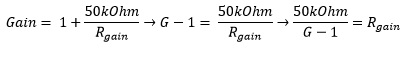
\includegraphics[width=1\textwidth]{Figurer/omskrivningtilgain}
\end{figure}

Herefter kan den ohmske værdi af *Rgain* bestemmes.\\

\begin{figure}[H]
	\centering
	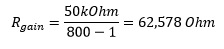
\includegraphics[width=1\textwidth]{Figurer/udregningafgain}
\end{figure}

\subsection{Design af analogfilter}
Filteret skulle realiseres som et aktivt 2. ordens lavpasfilter med båndbredde på 50 Hz af typen Sallen-Key med unity gain (se \ref{fig:Filter}). Filteret skulle designes som et Butterworth filter med cut off frekvens på 50 Hz. C2 skulle vælges til 680 nF og R1 = R2. Operationsforstærkeren skal være af typen OP27.  

\begin{figure}[H]
	\centering
	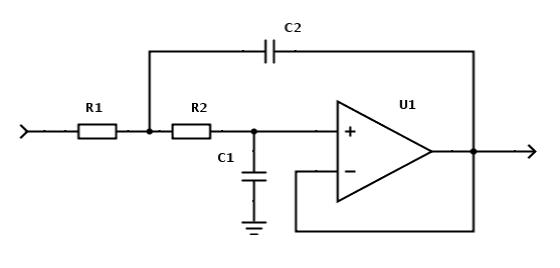
\includegraphics[width=1\textwidth]{Figurer/FilterDesign}
	\caption{Unity gain 2. ordens Sallen-Key lavpas konfiguration}
	\label{fig:Filter}
\end{figure}

Der blev valgt en dæmpningsfaktor på 1, da det ville være mest optimalt med et kritisk dæmpet signal. Ud fra hjemmesiden\footnote{http://sim.okawa-denshi.jp/en/OPseikiLowkeisan.htm} fandt vi overføringsfunktionen for Sallen-Kay lavpasfiltret:

\begin{figure}[H]
	\centering
	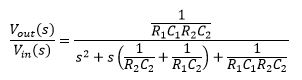
\includegraphics{Figurer/ligning1}
	\label{fig:lign1}
\end{figure}

Da det er blevet opgivet at $R1=R2$, kan overføringsfunktionen forkortes: 

\begin{figure}[H]
	\centering
	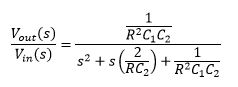
\includegraphics[width=1\textwidth]{Figurer/ligning2}
\end{figure}

Dernæst sammenlignes med standardformlen for overføringsfunktionen for et andet ordens filter.

\begin{figure}[H]
	\centering
	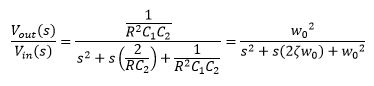
\includegraphics[width=1\textwidth]{Figurer/ligning3}
	\label{fig:lign3}
\end{figure}

Ud fra dette kan regnes komponentværdierne for R, idet

\begin{figure}[H]
	\centering
	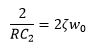
\includegraphics[width=1\textwidth]{Figurer/ligning4}
	\label{fig:lign4}
\end{figure}

Ved hjælp af mathcad isoleres R.

\begin{figure}[H]
	\centering
	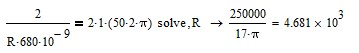
\includegraphics[width=1\textwidth]{Figurer/ligning5}
	\label{fig:lign5}
\end{figure}

Dernæst kan komponentværdien for C1 udregnes, idet:

\begin{figure}[H]
	\centering
	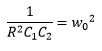
\includegraphics[width=1\textwidth]{Figurer/ligning6}
	\label{fig:lign6}
\end{figure}

Ved hjælp af mathcad isoleres C1. 

\begin{figure}[H]
	\centering
	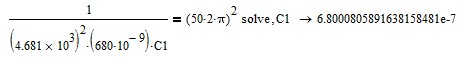
\includegraphics[width=1\textwidth]{Figurer/ligning7}
	\label{fig:lign7}
\end{figure}

Derved er komponentværdierne for kredsløbet fundet og de ses indskrevet på \ref{fig:Filter}. 

\begin{figure}[H]
	\centering
	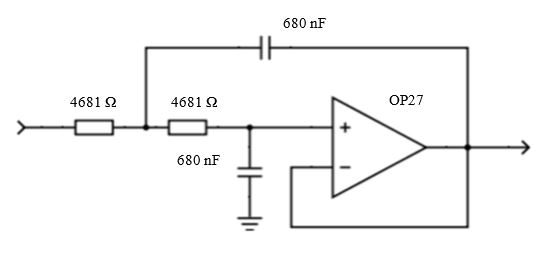
\includegraphics[width=1\textwidth]{Figurer/FilterDesignMedKomponentvaerdier}
	\caption{Unity gain 2. ordens Sallen-Key lavpas konfiguration med indsatte komponentværdier.}
	\label{fig:Filter_K}
\end{figure}

Generelt er et unity gain Sallen-Key filter med equivalente capacitorer og equivalente resistore kritisk dæmpet dvs. en kvalitets faktor på 1/2. Dette kan også ses når komponentværdierne indsættes i ”Sallen-Key Low-pass Filter Design Tool”\footnote{http://sim.okawa-denshi.jp/en/OPseikiLowkeisan.htm}. Desuden ses bodeplottet nedenfor:

\begin{figure}[H]
	\centering
	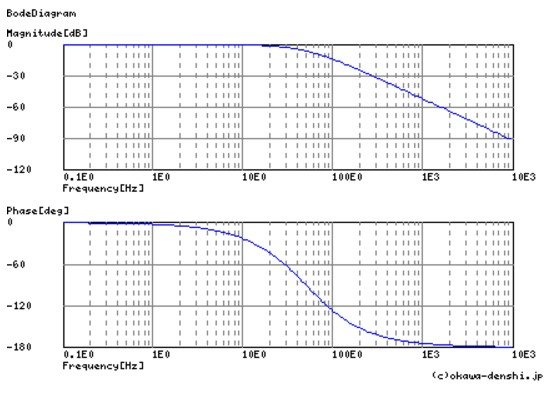
\includegraphics[width=1\textwidth]{Figurer/Bodeplot}
	\caption[]{Bodeplot af overføringsfunktionen\footnotemark}
	\label{fig:Bodeplot}
\end{figure}
\footnotetext{http://sim.okawa-denshi.jp/en/OPseikiLowkeisan.htm}


\subsection{Grænseflader}

\section{Software arkitektur}

\subsection{GUI}

\subsection{UML klassediagram}


\subsection{Appliktationsmodel}

\subsubsection{Klassediagram}

\begin{figure}[H]
	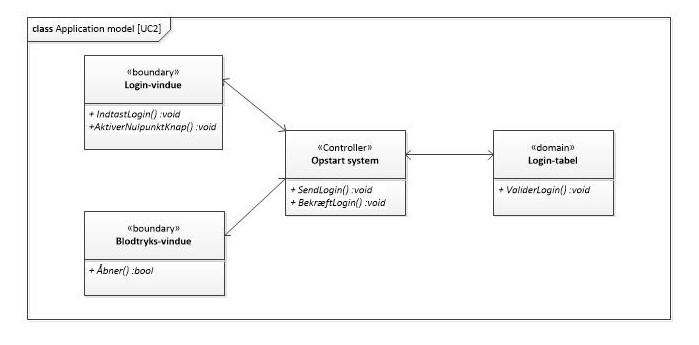
\includegraphics[width=1\textwidth]{Figurer/classAppModelUC2}
	\caption{Klassediagram UC 2}
	\label{classApp UC2}
\end{figure}

\begin{figure}[H]
	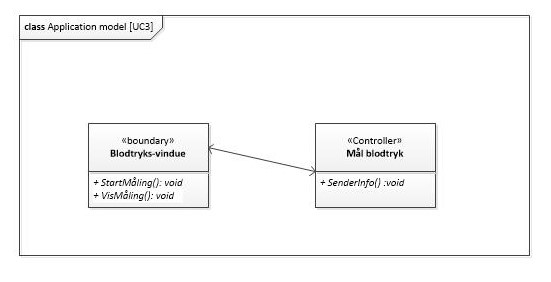
\includegraphics[width=1\textwidth]{Figurer/classAppModelUC3}
	\caption{Klassediagram UC 3}
	\label{classApp UC3}
\end{figure}

\begin{figure}[H]
	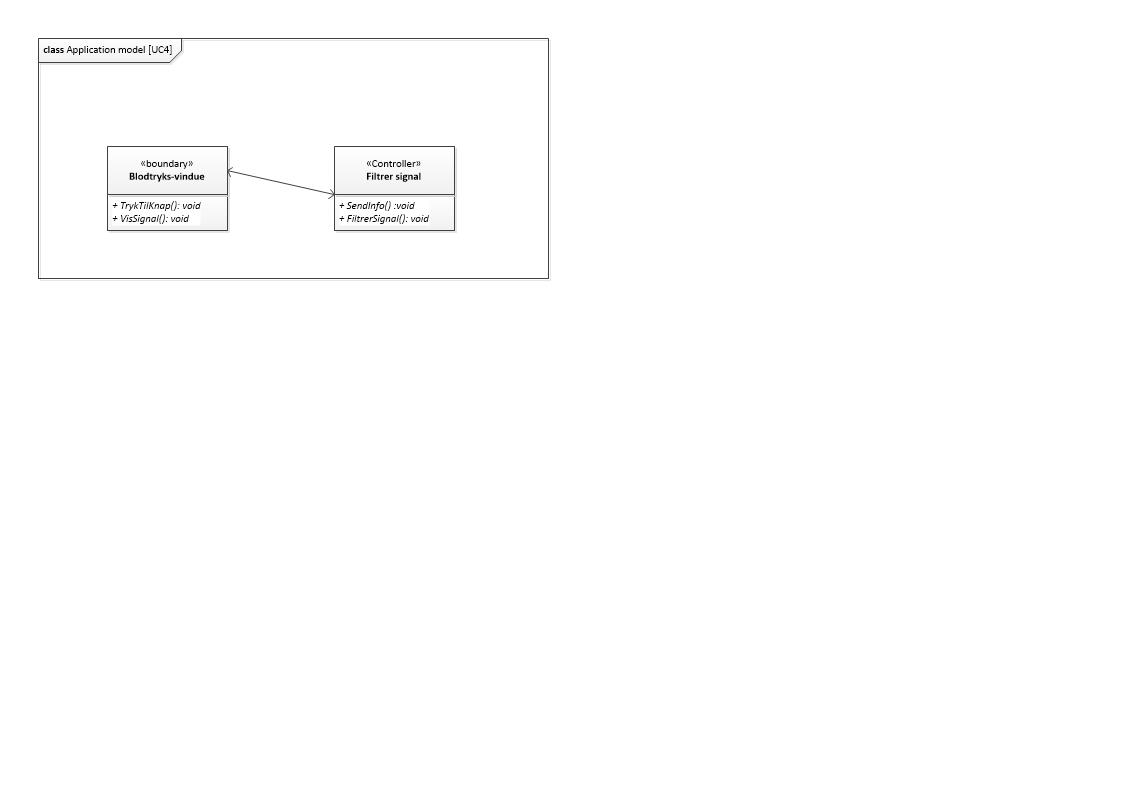
\includegraphics[width=1\textwidth]{Figurer/classAppModelUC4}
	\caption{Klassediagram UC 4}
	\label{classApp UC4}
\end{figure}

\begin{figure}[H]
	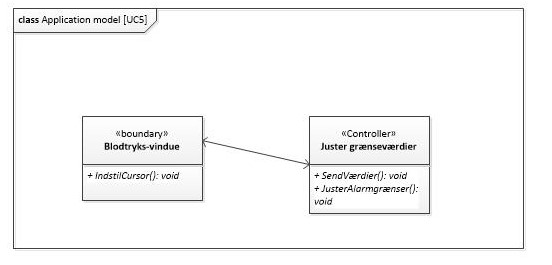
\includegraphics[width=1\textwidth]{Figurer/classAppModelUC5}
	\caption{Klassediagram UC 5}
	\label{classApp UC5}
\end{figure}

\begin{figure}[H]
	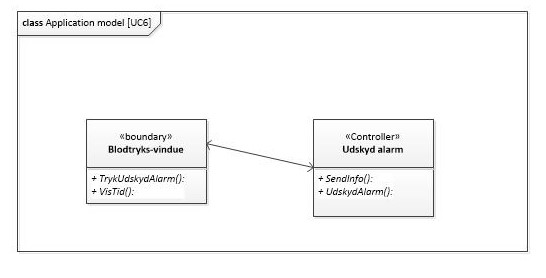
\includegraphics[width=1\textwidth]{Figurer/classAppModelUC6}
	\caption{Klassediagram UC 6}
	\label{classApp UC6}
\end{figure}

\begin{figure}[H]
	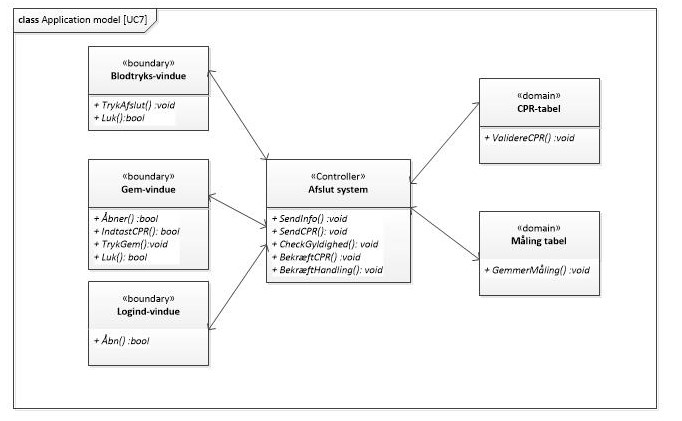
\includegraphics[width=1\textwidth]{Figurer/classAppModelUC7}
	\caption{Klassediagram UC 7}
	\label{classApp UC7}
\end{figure}



\subsubsection{Domænemodel}

\subsubsection{Sekvensdiagram}
\begin{figure}[H]
	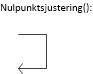
\includegraphics[width=1\textwidth]{Figurer/sdAppModelUC2}
	\caption{Sekvensdiagram UC2}
	\label{sd UC2}
\end{figure}

\begin{figure}[H]
	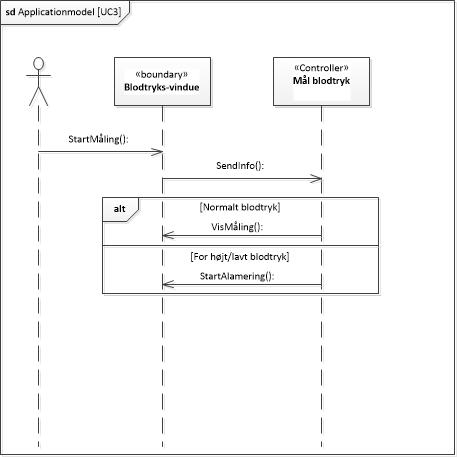
\includegraphics[width=1\textwidth]{Figurer/sdAppModelUC3}
	\caption{Sekvensdiagram UC3}
	\label{sd UC3}
\end{figure}

\begin{figure}[H]
	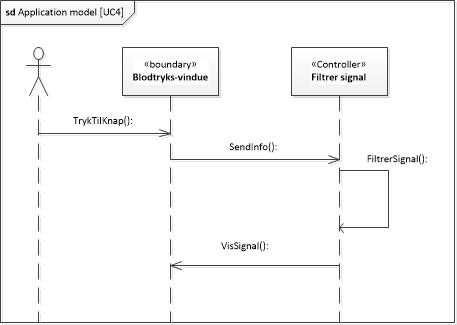
\includegraphics[width=1\textwidth]{Figurer/sdAppModelUC4}
	\caption{Sekvensdiagram UC4}
	\label{sd UC4}
\end{figure}

\begin{figure}[H]
	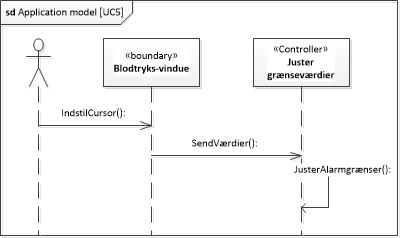
\includegraphics[width=1\textwidth]{Figurer/sdAppModelUC5}
	\caption{Sekvensdiagram UC5}
	\label{sd UC5}
\end{figure}

\begin{figure}[H]
	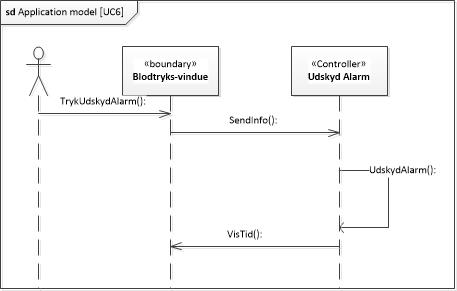
\includegraphics[width=1\textwidth]{Figurer/sdAppModelUC6}
	\caption{Sekvensdiagram UC6}
	\label{sd UC6}
\end{figure}

\begin{figure}[H]
	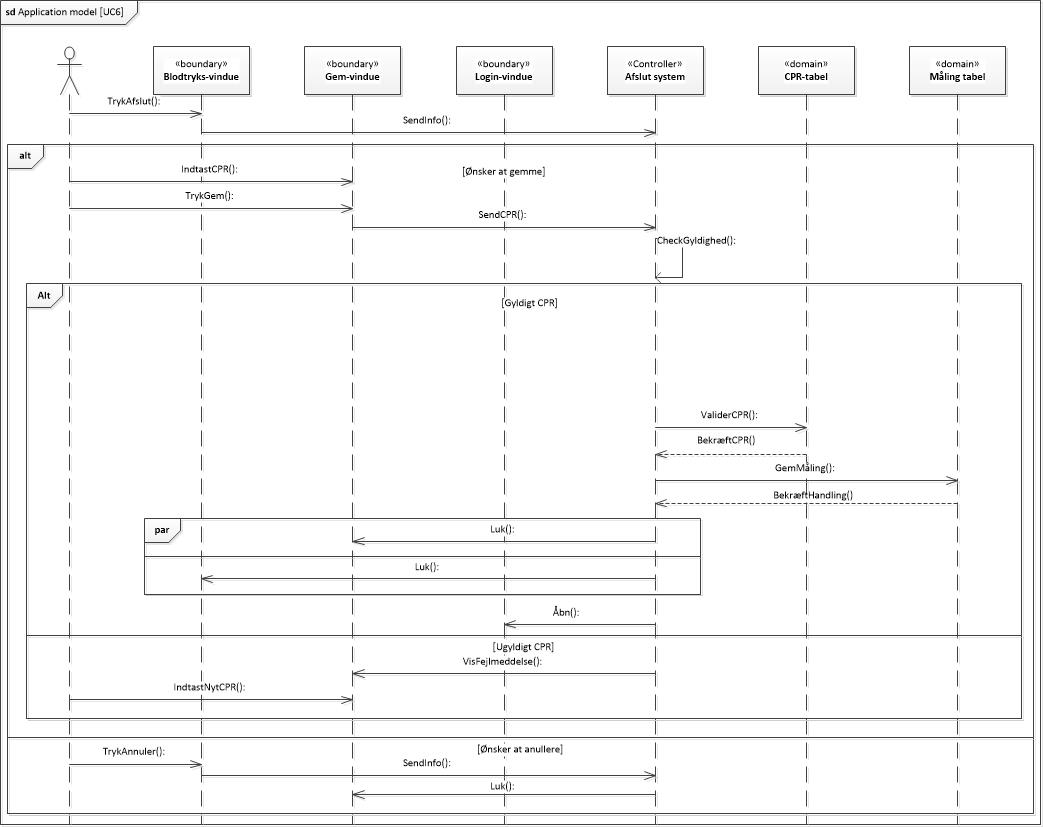
\includegraphics[width=1\textwidth]{Figurer/sdAppModelUC7}
	\caption{Sekvensdiagram UC7}
	\label{sd UC7}
\end{figure}

\subsubsection{Opdateret Klassediagram}

\section{Software implementering}
 
\subsection{Visning af EKG-signal}

\subsection{Analyse}

\subsection{Testprogram}

\subsection{Lagring i database} 

\subsubsection{Offentlig database}

\subsubsection{Privat database}







